\documentclass{article}
\usepackage{tikz}
\usepackage{fullpage}
\usepackage{amsmath,amsfonts,amssymb,stmaryrd}

\title{Projet de Logique: Loup Chèvre Choux}
\author{Waxin Alban, Le Meur Quentin, Laurin Guillaume, Sansané Hugo, Said Yacine}

\setlength{\topmargin}{-1.5cm}
\setlength{\textheight}{25cm}
\setlength{\textwidth}{18cm}
\setlength{\oddsidemargin}{-1.5cm}
\setlength{\evensidemargin}{50cm}

\newcommand{\R}{\mathbb{R}}
\newcommand{\C}{\mathbb{C}}
\newcommand{\N}{\mathbb{N}}
\newcommand{\Q}{\mathbb{Q}}
\newcommand{\Z}{\mathbb{Z}}
\newcommand{\K}{\mathbb{K}}
\newcommand{\M}{\mathcal{M}}


\begin{document}
\maketitle\newpage
\section{Sujet}
\subsection{choix et règles}
L’énigme du loup, de la chèvre et du chou est une énigme de type “Passage de pont” dont les origines remontes au IXeme siècle.
Le but est de faire traverser 4 entités : un fermier , un loup, une chèvre et un choux d’une rive gauche a une rive droite a l’aide d’un bateau avec les contraintes suivantes :

\begin{itemize}
  \item  Il est impossible de transporter plus de 2 entités en même temps sur le bateau
  \item  le bateau doit être conduit par le fermier uniquement
  \item  il est impossible de laisser le loup et la chèvre seul sans le fermier
  \item  il est impossible de laisser la chèvre et le choux seul sans le fermier
\end{itemize}

\subsection{Etudes préliminaires}
Il existe des variantes a l’énigme du loup, de la chèvre et du chou avec d’autres entités ou un nombre de place différents dans le bateau, nous nous conterons dans la plus grande partie de notre sujet sur la version classique de l’énigme puis nous émettrons des axes d’amelioration pour généraliser la solution.
Une étude préliminaire nous a permis de determiner les nécessités suivantes :
\begin{itemize}
  \item Notre logique doit permettre de modéliser l’aspect temporel du problème
  \item Notre logique doit permettre de visualiser les états de chaque berges
\end{itemize}

\section{Définition de la logique}
\subsection{Formalisation}
Nous utiliserons des fonctions constantes pour modéliser nos entités et une fonction prenant en paramètre une entité
\begin{itemize}
  \item $f$ : pour l’entité fermier
  \item $l$ : pour l’entité Loup
  \item $c$ : pour l’entité Chèvre
  \item $b$ : pour l’entité choux
\end{itemize}
Nous utiliserons une infinité de prédicats représentant trois informations à un moment t donné
\begin{itemize}
  \item $RG_t(x)$ : x est sur la rive gauche a l’itération t
  \item $RD_t(x)$ : x est sur la rive droite a l’itération t
  \item $S_t(x)$ : x est en sécurité a l’itération t
\end{itemize}
Ainsi qu'un prédicat réprésentant la situation prédateur proie :
$M(x,y)$ : x mange y\\
Le bateau ne sera pas modélisé car il ne représente que la transition entre deux itérations
\subsection{Langage}
Nous avons décider de choisir une logique du Premier Ordre, car elle permet de décrire les personnages
à l’aide de termes d’arrité 0 et les états des règles de sécurité par des prédicats \\
\\
Soit $\mathcal{L} = (\mathcal{F} ,\mathcal{P} ,\mathcal{C} ,\mathcal{Q} )$
\begin{itemize}
  \item $ \mathcal{F} := \{(f,0),(l,0),(c,0),(b,0)\}$
  \item $ \mathcal{P} := \{\forall i \in \N,(S_i,1),(RG_i,1),(RD_i,1),(P,0),(G,0)(M,2)\} $
  \item $ \mathcal{C} := \{(\bot , 0),(\top , 0),(\neg , 1), (\vee , 2), (\wedge , 2), (\rightarrow , 2)\}$
  \item $ \mathcal{Q} := \{\exists, \forall \}$
\end{itemize}
\subsection{Syntaxe}
Termes : \\
$t := x|f|l|c|b|m(x)$ \\
Formules : \\
$A := \forall i \in\N, S_i(t)|RD_i(t)|RG_i(t)|P_i|G_i|M(t,t)|(t=t)| \bot|\top|\neg A|A\vee A|A\wedge A|A \rightarrow A$

\subsection{Notations}
$ a \leftrightarrow b = (a \rightarrow b) \wedge  (b \rightarrow a)$
\subsection{Interprétation}
Domaine d'Interprétation : $D = \{f,l,c,b\}$
\begin{itemize}
  \item $\forall x,y , M(x,y) = \neg(x=f) \wedge \neg(x=b) \wedge (x=l \leftrightarrow y=c) \wedge (x=c \leftrightarrow y=b)$
  \item $\forall x , S_t(x) = (RG_t(x) \to (\forall y , RG_t(y) \to \neg M(y,x) )) \wedge (RD_t(x) \to (\forall y , RD_t(y) \to \neg M(y,x) )) $
  \item[$ \to $] État initial :
    \begin{itemize}
      \item[$ \to $] Rive Gauche :
      \item $ RG_0(f) = \top $
      \item $ RG_0(l) = \top $
      \item $ RG_0(c) = \top $
      \item $ RG_0(b) = \top $
      \item[$ \to $] Rive Droite
      \item $ RD_0(f) = \bot $
      \item $ RD_0(l) = \bot $
      \item $ RD_0(c) = \bot $
      \item $ RD_0(b) = \bot $
    \end{itemize}

\end{itemize}


\subsection{Axiomatisation}
Soit A, B et C des variables propositionnelles.
% \begin{enumerate}
%   \item $ (A \wedge A) \leftrightarrow  A$ : idempotence
%   \item $ (A \vee A) \leftrightarrow  A$ : idempotence
%   \item $ (A \wedge B) \leftrightarrow  (B \wedge A)$ : commutativité
%   \item $ (A \vee B) \leftrightarrow  (B \vee A)$ : commutativité
%   \item $ (A \wedge (B \wedge C)) \leftrightarrow  ((A \wedge B) \wedge C)$ : associativité
%   \item $ (A \vee (B \vee C)) \leftrightarrow  ((A \vee B) \vee C)$ : associativité
%   \item $ ((A \wedge (B \vee C)) \leftrightarrow ((A \wedge B) \vee (A \wedge C)))$ : distributivité
%   \item $ ((A \vee (B \wedge C)) \leftrightarrow ((A \vee B) \wedge (A \vee C))) $ : distributivité
%   \item $ (A \wedge (A \vee B)) \leftrightarrow  A$ : absorption
%   \item $ (A \vee (A \wedge B)) \leftrightarrow  A$ : absorption
%   \item $ \neg (A \vee B) \leftrightarrow \neg A \wedge \neg B$ : lois de de Morgan
%   \item $ \neg (A \wedge B) \leftrightarrow \neg A \vee \neg B$ : lois de de Morgan
%   \item $ A \wedge \top \leftrightarrow A$
%   \item $ A \vee \bot \leftrightarrow A$
%   \item $ A \wedge \bot \leftrightarrow \bot$
%   \item $ A \vee \top \leftrightarrow \top$
%   \item $ (A \rightarrow B) \leftrightarrow (\neg A \rightarrow \neg B)$ : contraposée
% \end{enumerate}
\begin{itemize}
  \item Tautologies. Les tautologies de la logique du premier ordre
        sont construites comme suit
  \item[] \begin{enumerate}
      \item
            Soit $A(p_1, \dots , p_n)$ une tautologie de la logique propositionnelle
      \item Prendre n formules de la logique du premier ordre $B_1, \dots , B_n$
      \item Substituer la variable propositionnelle $p_1$ par la formule $B_1$, \dots, $p_n$ par la formule $B_n$
      \item La formule $A(B_1, \dots , B_n)$ est une tautologie de la logique du premier ordre.
    \end{enumerate}
  \item Les axiomes des quantificateurs.
  \item[] \begin{itemize}
      \item $\exists x, A \leftrightarrow \neg \forall x, \neg A$
      \item $\forall x,(A \rightarrow B) \rightarrow (A \rightarrow \forall x, B)$ où x est une variable qui n’a pas d’occurrence libres dans A.
      \item $(\forall x, A) \rightarrow A_{t / x}$ où t est un terme tel que aucune aucune occurrence libre de x ne se trouve dans le champ d'un quantificateur liant une variable de t
    \end{itemize}
\end{itemize}
\newpage
\subsection{Axiomes}
\begin{itemize}
  \item \small On définit une infinité d'axiome représentant chacun l'état de sécurité d'une entité à un moment t donné:
        \begin{align*}
          a_1:= \forall x,S_t(x) & \leftrightarrow  (\forall y, \neg M(y,x)) \\ &\vee (\exists y , M(y,x) \wedge ((RG_t(x)\wedge RD_t(y)) \vee (RD_t(x)\wedge RG_t(y)))\\
                                 & \vee (RG_t(x) \wedge RG_t(f))             \\
                                 & \vee (RD_t(x) \wedge RD_t(f))
        \end{align*}
  \item On définit le fait que l'on ne puisse pas avoir un gain et une perte en même temps\\
        $a_2:= (G_t \to \neg P_t)$
  \item On définit ce qui rend un chemin perdant, c'est à dire avoir perdu à l'itération précédente ou avoir une entité qui n'est pas en sécurité à l'itération courante\\
        $a_3:= P_t \leftrightarrow \exists x, \neg S_t(x) \vee P_{(t-1)}$
  \item On définit un chemin gagnant par le fait qu'a un moment on aie les quatres entités sur la rive droite\\
        $a_4:= G_t \leftrightarrow RD_t(l) \wedge RD_t(f) \wedge RD_t(c) \wedge RD_t(b) \leftrightarrow  \forall x, RD_t(x)$
  \item On définit une infinité d'axiome représentant l'impossibilité d'etre sur deux rives en même temps:\\
        $a_5 := \forall x ,RG_t(x) \leftrightarrow \neg RD_t(x)$
  \item Le Loup et le fermier n'ont pas de pédateurs ils sont donc tout le temps en sécurité\\
        $a_6 := S_t(f) \wedge S_t(l)$
  \item On définit la variation de population des rives à chaque voyage\\
        pour t=2n ,
\end{itemize}

\section{Problème et étude}
\subsection{Problème}


\section*{Graphe des chemins possibles }

%:-+-+-+- Engendré par : http://math.et.info.free.fr/TikZ/Arbre/
\begin{center}
  % Racine en Haut, développement vers le bas
  \begin{tikzpicture}[xscale=0.9,yscale=0.9]
    % Styles (MODIFIABLES)
    \tikzstyle{fleche}=[->,>=latex,thick]
    \tikzstyle{noeud}=[fill=white,circle,draw]
    \tikzstyle{feuille}=[fill=red!20,circle,draw]
    \tikzstyle{feuilleF}=[fill=lime!20,circle,draw]
    \tikzstyle{feuilleR}=[fill=orange!20,circle,draw]
    \tikzstyle{etiquette}=[midway,fill=white,draw]
    % Dimensions (MODIFIABLES)
    \def\DistanceInterNiveaux{2.5}
    \def\DistanceInterFeuilles{2}
    % Dimensions calculées (NON MODIFIABLES)
    \def\NiveauA{(-0)*\DistanceInterNiveaux}
    \def\NiveauB{(-1.8571428571428572)*\DistanceInterNiveaux}
    \def\NiveauC{(-3.571428571428571)*\DistanceInterNiveaux}
    \def\NiveauD{(-5.142857142857142)*\DistanceInterNiveaux}
    \def\NiveauE{(-6.571428571428571)*\DistanceInterNiveaux}
    \def\NiveauF{(-7.857142857142857)*\DistanceInterNiveaux}
    \def\NiveauG{(-9)*\DistanceInterNiveaux}
    \def\NiveauH{(-10)*\DistanceInterNiveaux}
    \def\InterFeuilles{(1)*\DistanceInterFeuilles}
    % Noeuds (MODIFIABLES : Styles et Coefficients d'InterFeuilles)
    \node[feuilleR] (R) at ({(3.5)*\InterFeuilles},{\NiveauA}) {$FLCB|$};
    \node[feuille] (Ra) at ({(0)*\InterFeuilles},{\NiveauB}) {$LCB|F$};
    \node[feuille] (Rb) at ({(1)*\InterFeuilles},{\NiveauB}) {$CL|FB$};
    \node[feuille] (Rc) at ({(2)*\InterFeuilles},{\NiveauB}) {$CB|FL$};
    \node[noeud] (Rd) at ({(5)*\InterFeuilles},{\NiveauB}) {$LB|FC$};
    \node[noeud] (Rda) at ({(5)*\InterFeuilles},{\NiveauC}) {$FLB|C$};
    \node[noeud] (Rdaa) at ({(4)*\InterFeuilles},{\NiveauD}) {$B|FCL$};
    \node[feuille] (Rdaaa) at ({(3)*\InterFeuilles},{\NiveauE}) {$BF|CL$};
    \node[noeud] (Rdaab) at ({(4.5)*\InterFeuilles},{\NiveauE}) {$BFC|L$};
    \node[feuille] (Rdaaba) at ({(4)*\InterFeuilles},{\NiveauF}) {$BC|FL$};
    \node[noeud] (Rdaabb) at ({(5)*\InterFeuilles},{\NiveauF}) {$C|LFB$};
    \node[noeud] (Rdaabba) at ({(5)*\InterFeuilles},{\NiveauG}) {$FC|LB$};
    \node[feuilleF] (Rdaabbaa) at ({(5)*\InterFeuilles},{\NiveauH}) {$|FCLB$};
    \node[noeud] (Rdab) at ({(6.5)*\InterFeuilles},{\NiveauD}) {$L|FCB$};
    \node[feuille] (Rdaba) at ({(7)*\InterFeuilles},{\NiveauE}) {$LF|CB$};
    \node[noeud] (Rdabb) at ({(6)*\InterFeuilles},{\NiveauE}) {$FCL|B$};
    \node[feuille] (Rdabba) at ({(6)*\InterFeuilles},{\NiveauF}) {$LC|FB$};
    % Arcs (MODIFIABLES : Styles)
    \draw[fleche] (R)--(Ra) ;
    \draw[fleche] (R)--(Rb) ;
    \draw[fleche] (R)--(Rc) ;
    \draw[fleche] (R)--(Rd) ;
    \draw[fleche] (Rd)--(R) ;

    \draw[fleche] (Rd)--(Rda) ;
    \draw[fleche] (Rda)--(Rd) ;

    \draw[fleche] (Rda)--(Rdaa) ;
    \draw[fleche] (Rdaa)--(Rda) ;
    \draw[fleche] (Rdab)--(Rda) ;
    \draw[fleche] (Rdaa)--(Rdaaa) ;
    \draw[fleche] (Rdaab)--(Rdaa) ;
    \draw[fleche] (Rdabb)--(Rdab) ;
    \draw[fleche] (Rdaa)--(Rdaab) ;
    \draw[fleche] (Rdaabb)--(Rdaab) ;
    \draw[fleche] (Rdaabb)--(Rdabb) ;
    \draw[fleche] (Rdaabba)--(Rdaabb) ;

    \draw[fleche] (Rdaab)--(Rdaaba) ;
    \draw[fleche] (Rdaab)--(Rdaabb) ;
    \draw[fleche] (Rdaabb)--(Rdaabba) ;
    \draw[fleche] (Rdaabba)--(Rdaabbaa) ;
    \draw[fleche] (Rda)--(Rdab)  ;
    \draw[fleche] (Rdab)--(Rdaba)  ;
    \draw[fleche] (Rdab)--(Rdabb) ;
    \draw[fleche] (Rdabb)--(Rdabba) ;
    \draw[fleche] (Rdabb)--(Rdaabb) ;
  \end{tikzpicture}
\end{center}
%:-+-+-+-+- Fin


\section*{Preuve des chemins gagnants}

Donc par interpretation des états initiaux:

\subparagraph*{Pour t = 0:}
on a $(RG_0(c) \wedge RG_0(f) \wedge RG_0(l) \wedge RG_0(b)) \wedge (\neg RD_0(c) \wedge \neg RD_0(f) \wedge \neg RD_0(l) \wedge \neg RD_0(b))\\ $
$\leftrightarrow RG_0(c) \wedge RG_0(f) \wedge RG_0(l) \wedge RG_0(b)$ par axiome 5\\

or
\begin{align*}
  RG_0(c) \wedge RG_0(f) \wedge RG_0(l) \wedge RG_0(b) &
  \leftrightarrow RG_0(f) \wedge (RG_0(f) \wedge RG_0(c) \wedge RG_0(b) \wedge RG_0(l))                                                                                                           \\
                                                       & \leftrightarrow [RG_0(f) \wedge RG_0(f)] \wedge [RG_0(f) \wedge RG_0(c)] \wedge [RG_0(f) \wedge RG_0(b)] \wedge [RG_0(f) \wedge RG_0(l)] \\
                                                       & \leftrightarrow \forall x, RG_0(f) \wedge RG_0(x)                                                                                        \\
                                                       & \leftrightarrow \forall x, S_0(x) \text{ par axiome 1}                                                                                   \\
                                                       & \leftrightarrow P_0 = \bot \text{ par axiome 3}
\end{align*}
\begin{align*}
  RG_0(c) \wedge RG_0(f) \wedge RG_0(l) \wedge RG_0(b) &
  \leftrightarrow RG_0(f) \wedge (RG_0(f) \wedge RG_0(c) \wedge RG_0(b) \wedge RG_0(l))                               \\
                                                       & \rightarrow \exists x , RG_0(x)                              \\
                                                       & \leftrightarrow \exists x, \neg RD_0(x) \text{ par axiome 5} \\
                                                       & \leftrightarrow \neg (\forall x, RD_0(x))                    \\
                                                       & \leftrightarrow G = \bot \text{ par axiome 4}                \\
\end{align*}
Donc le jeu peut continuer

\subparagraph*{Pour t = 1:}

Pour cette itération il existe quatre chemins possible

Dénotons la structure d'un voyage:\\
Soit x l'élément qui part avec le fermier (f)\\
la situation se traduit alors par :\\
$(\forall y , \neg(x = y \vee y = f) \rightarrow RG_1(y)) \wedge (RD_1(x) \wedge RD_1(f))$
Démontrons maintenant la condition qui fait d'un chemin une défaite

Montrons le maintenant pour les cas de notre étude\\
Pour $x=l$
on a alors $RG(c)\wedge RG(b) \wedge RD(f) \wedge RD(l)$\\
or $(m(c)=b) \wedge RD(f) \rightarrow \neg S_1(b) \rightarrow P = \top$



\end{document}
